\scanpage{78}

% upper left, hexagon and three marks below
\figure{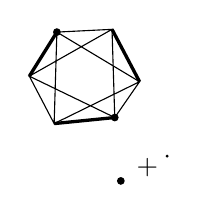
\begin{tikzpicture}[scale=.7]
\coordinate (a) at (-1,0);\coordinate (b) at (-.5,.8);\coordinate (c) at (.5,.85);\coordinate (d) at (1,-.1);\coordinate (e) at (.55,-.75);\coordinate (f) at (-.55,-.86);
\draw (a)--(b)--(c)--(d)--(e)--(f)--cycle (a)--(c)--(e)--cycle (b)--(d)--(f)--cycle;
\draw[very thick] (a)--(b) (c)--(d) (e)--(f);\fill (b) circle (2pt) (e) circle (2pt) (.66,-1.9) circle (2pt);\node at (1.14,-1.65) {$+$};\fill (1.5,-1.45) circle (.8pt);
\end{tikzpicture}}

% top, second sketch
\diagram{\begin{tikzcd}[ampersand replacement=\&,row sep=small,execute at end picture={\draw[thin] ([xshift=-8pt]r.north west) -- ([xshift=-14pt]g.south west);}]
t_1\arrow[r,dash]\arrow[dr,dash]\arrow[ddr,dash]\&|[alias=r]| \alpha\\
t_2\arrow[ur,dash]\arrow[r,dash]\arrow[dr,dash]\&\beta\\
t_0\,{\times}\& |[alias=g]| \gamma
\end{tikzcd}}

% top centre, two short rows
\[
\begin{array}{cccc}
\deleted{\unsure{12|13}}&\unsure{f_{14}}&f_{15}&f_{16}\\
&f_{24}&f_{25}&f_{26}
\end{array}
\]

% top centre, three rows and left arrow
\diagram{\begin{tikzcd}[ampersand replacement=\&,column sep=small,row sep=small]
(t_1,\alpha)\arrow[dr,dash]\arrow[drr,dash]\&(t_1,\beta)\&(t_1,\gamma)\\
(t_2,\alpha)\&(t_2,\beta)\&(t_2,\gamma)\\
(t_0,\alpha)\&(t_0,\beta)\&(\unsure{t_0|t_1},\gamma)\\
{}\&{}\arrow[l]\&
\end{tikzcd}}

% top right, heading and small isolated hexagon
$H$ un hexagone

% top right, by heading
\figure{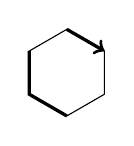
\begin{tikzpicture}[scale=.55]
\draw (90:1)--(30:1)--(-30:1)--(-90:1)--(-150:1)--(150:1)--cycle;
\draw[very thick,->] (90:1)--(30:1);\draw[very thick] (150:1)--(-150:1)--(-90:1);
\end{tikzpicture}}

% upper right, definitions and cardinalities
\[
\begin{aligned}
H_d&\quad\text{ens des diagonales = ens des codiagonales} &&3\\
H_t&\quad\text{ens des triangles inscrits} &&2\\
H_\omega&\quad\text{ens des orientations}\simeq\omega(H_d) &&\big\}2\quad\deleted{\unsure{H_\omega\simeq H_t\wedge\omega(H_d)}}\\
\inserted{H_{t*}}&\quad\inserted{\text{ens des triangles circonscrit}} &&2\\
H_s&\quad\text{ens des sommets}=H_d\times H_t &&6\\
H_{s*}&\quad\text{ens des côtés}=H_d\times H_{t*} &&6\\
H_r&\quad\text{ens des repères}\subset H_s\times H_d &&12\\[-3pt]
&&\text{rel. d'inc. }\text{''}&
\end{aligned}
\]

% under definitions, crossed row and inserted products
\[
\begin{aligned}
&\unsure{H_{r_1}|H_{r'}}\quad H_d\times H_d^{*}\times H_t\times H_{t*}\\
&\deleted{\unsure{H_{s**}|H_{r'}}\quad\text{ens des rep. \unsure{mut.} opp.}=6}\\
&H_{t\mathrm{ror}}=\text{triangles inscrits orientés}\qquad 4
\end{aligned}
\]

% centre and left, network of coverings
\diagram{\resizebox{\linewidth}{!}{\begin{tikzcd}[ampersand replacement=\&,column sep=2.8em,row sep=3.7em,cells={font=\scriptsize}]
\& {\substack{\mathrm{hex}+\mathrm{diag}\\\simeq\mathrm{tria}+\text{él. marqué}\\\simeq\text{couples de trièdres}\\\text{sécants (explicités!)}}}\arrow[d,"3"] \&
{\text{(échanges)}}\arrow[dl,dash]\arrow[d]\&\\
|[alias=A]|{\substack{\mathrm{tria}'=\mathrm{Hex}+\mathrm{diag}\\\mathrm{Hex}+\mathrm{codiag}\\=\text{bib. pliée}}}\arrow[d,"3"] \&
|[alias=B]|{\substack{\mathrm{tria}\simeq\mathrm{hex}\\=\mathrm{Hex}+\text{sommet}}}\arrow[l,"2" description,"\mathrm{opp}"']\arrow[d,"3"] \&
|[alias=C]|{\substack{\mathrm{hexor}\;(\mathrm{hex}+\text{orientation})\\\simeq\mathrm{triaor}\;(\text{trièd.}+\text{ordre circulaire})\\\simeq\omega((\mathrm{hex}+\mathrm{diag})/\mathrm{hex})}}\arrow[l,"2"]\&\\
|[alias=D]|{\deleted{\unsure{\mathrm{H}}}\mathrm{Hex}}\arrow[dd,"3"]\&|[alias=E]|{\substack{\mathrm{trtria}\\\simeq\omega(\mathrm{Hex}/\mathrm{triHex})\ (\mathfrak S_3\text{-tors sur }\mathrm{triHex})\\\simeq\mathrm{Hex}+\text{triangle inscr}\\\simeq\text{pav}+\unsure{\text{coor.}|\text{or.}}}}\arrow[l,"\deleted{\unsure{2}}\,2"']\&{\mathrm{hex}+\text{somm.}}\arrow[l]\arrow[d]\&
{\substack{\mathrm{hex}+\text{triangle inscrit orienté}\\\simeq\text{couples de trièdres orientées}\\\text{parallèles}}}\arrow[ul]\arrow[dl]\\
\&|[alias=F]|{\substack{\mathrm{triaor}'=\mathrm{Hex}\\+\text{rep mod opp}\\(\text{torseur sur }\mathrm{Hex}\\\text{de gpe }\mathfrak S_3)}}\arrow[to=A,"2"]\arrow[d]\arrow[dd,bend left=15,"3"]\&|[alias=G]|{\substack{\deleted{\unsure{\mathrm{Hexrep}}}=\mathrm{Hex}+\mathrm{rep}\simeq\text{couple de trièd. \unsure{liées|fibrées}}\simeq\mathrm{hex}+\text{trièd. marqué}\\\simeq\text{couple de trièdres par.}\\\simeq\mathrm{hex}+\text{``triangle inscr''}\\(\text{torseur sur Hex de gpe }\mathfrak S_3\times\mathfrak S_2)\\\text{torseur sur trtria de gpe }\mathfrak S_3\\\simeq\text{torseur sur triaor gpe }\mathfrak S_2}}\arrow[l,"\mathrm{opp}"']\arrow[to=B,"2"]\arrow[dd]\&\\
{\substack{\deleted{\mathrm{triHex}}\\\mathrm{triHex}}}\&-\mathrm{Pav}\arrow[l,"3"']\&\&\\
\&{\substack{\mathrm{Hexor}\simeq\omega(\mathrm{tria}'/\mathrm{Hex})\\=\mathrm{Hex}+\mathrm{or.}}}\arrow[to=D,"2"]\&
{\substack{\mathrm{trortria}\\\simeq\mathrm{Hex}+\mathrm{tr.or.}\\\text{inscr.}}}\arrow[l,"2"']\arrow[to=E,"2"]\&
\end{tikzcd}}}

% lower right, star and circumscribed sketch
\figure{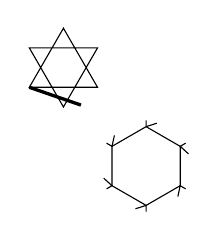
\begin{tikzpicture}[scale=.5]
\draw (90:1)--(210:1)--(330:1)--cycle (150:1)--(270:1)--(30:1)--cycle;\draw[very thick] (210:1)--(-65:1.05);
\begin{scope}[shift={(2.1,-2.5)}]\draw (90:1)--(30:1)--(-30:1)--(-90:1)--(-150:1)--(150:1)--cycle;
\foreach \a in {90,30,-30,-90,-150,150}{\draw (\a:1.16)--(\a:1)--({\a-14}:1.12);}\end{scope}
\end{tikzpicture}}

% bottom middle, list of subgroups
$\mathfrak S_3\times\mathfrak S_2$

$7$ ss-gpes d'indice $2$ \unsure{(3 de ?)|(3 classes)}

$3$ ss-gpes d'indice $4$ (\unsure{conj})

$3$ sous-gpes d'indice $6$ (\inserted{non} conjugués)

% lower right, large marked hexagon over small diagram
\figure{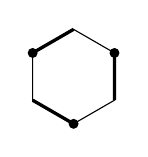
\begin{tikzpicture}[scale=.6]
\draw (90:1)--(30:1)--(-30:1)--(-90:1)--(-150:1)--(150:1)--cycle;
\draw[very thick] (150:1)--(90:1) (30:1)--(-30:1) (-90:1)--(-150:1);
\foreach \a in {150,30,-90}{\fill (\a:1) circle (3pt);}\end{tikzpicture}}

% bottom right, diagram
\diagram{\begin{tikzcd}[ampersand replacement=\&,row sep=small,column sep=small,cells={font=\scriptsize}]
\&H_s\arrow[ddl]\arrow[ddd]\&\&H_r\;\mathfrak S_3\times\mathfrak S_2\arrow[ll]\arrow[dll]\arrow[ddl]\arrow[ddd]\\
\&\mathfrak S_3 H_{r_1}\arrow[dl]\arrow[ddd]\&\&\\
H_d\arrow[ddd]\&\&H_{s*}\arrow[ll]\arrow[ddd]\&\\
\&H_t\arrow[ddl]\&\&H_{t\mathrm{ror}}\arrow[ll]\arrow[dll]\arrow[ddl]\\
\&H_\omega\arrow[dl]\&\&\\
e\&\&H_{t*}\arrow[ll]\&
\end{tikzcd}}

% archive sheet number: 77
